\documentclass[aspectratio=169]{beamer}
\usepackage{fontspec,tikz,graphicx,xcolor}
\setmainfont{NimbusRoman-Regular.otf}[Path=/usr/share/fonts/opentype/urw-base35/,BoldFont=NimbusRoman-Bold.otf,ItalicFont=NimbusRoman-Italic.otf,BoldItalicFont=NimbusRoman-BoldItalic.otf]
\setsansfont{NimbusRoman-Regular.otf}[Path=/usr/share/fonts/opentype/urw-base35/,BoldFont=NimbusRoman-Bold.otf,ItalicFont=NimbusRoman-Italic.otf,BoldItalicFont=NimbusRoman-BoldItalic.otf]
\setbeamertemplate{navigation symbols}{}
\definecolor{bg}{HTML}{000000}\definecolor{ink}{HTML}{FFFFFF}\definecolor{yel}{HTML}{FFD45C}
\setbeamercolor{background canvas}{bg=bg}
\setbeamercolor{normal text}{fg=ink,bg=bg}
\setbeamersize{text margin left=0pt,text margin right=0pt}
\begin{document}
\begin{frame}[plain]
\begin{tikzpicture}[remember picture,overlay]
\node[anchor=north west,inner sep=0pt,text width=60.00000mm,align=left,text=ink,font=\fontsize{7.0866}{7.6535}\selectfont \bfseries ] at ([xshift=6.96000mm,yshift=-1.25000mm]current page.north west) {UFPB  ·  CEAR  ·  PPGER};
\node[anchor=north west,inner sep=0pt,text width=38.75000mm,align=left,text=ink,font=\fontsize{7.0866}{7.6535}\selectfont ] at ([xshift=114.00000mm,yshift=-1.25000mm]current page.north west) {SPGER0046  ·  03 DEZ 2026};
\draw[yel,line width=.12mm] ([xshift=6mm,yshift=-4.56mm]current page.north west)--([xshift=153.84mm,yshift=-4.56mm]current page.north west);
\node[anchor=north west,inner sep=0pt,text width=145.62500mm,align=left,text=ink,font=\fontsize{14.5275}{15.6897}\selectfont \bfseries ] at ([xshift=6.96000mm,yshift=-7.62500mm]current page.north west) {1.1 · GEOMETRIA SOLAR};
\node[anchor=north west,inner sep=0pt,text width=143.75000mm,align=left,text=yel,font=\fontsize{10.2756}{11.0976}\selectfont ] at ([xshift=7.44000mm,yshift=-17.50000mm]current page.north west) {A direção do Sol organiza a projeção do feixe direto.};
\node[anchor=north west,inner sep=0pt] at ([xshift=8.2139mm,yshift=-26.8750mm]current page.north west) {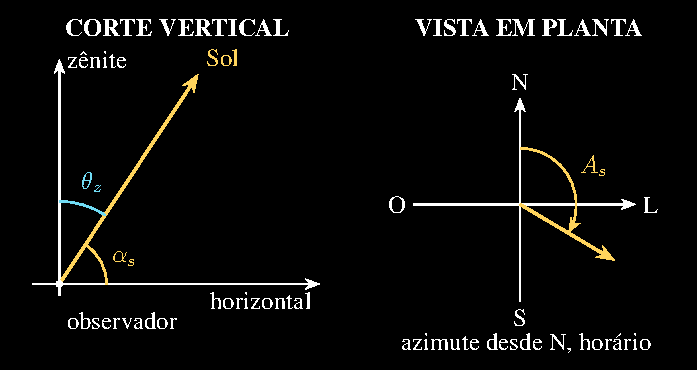
\includegraphics[width=86.0723mm,height=45.6250mm,keepaspectratio]{../figuras/D01_geometria.pdf}};
\node[anchor=north west,inner sep=0pt,text width=51.25000mm,align=left,text=yel,font=\fontsize{11.6929}{12.6283}\selectfont \bfseries ] at ([xshift=100.00000mm,yshift=-27.50000mm]current page.north west) {Ângulo zenital};
\node[anchor=north west,inner sep=0pt,text width=51.25000mm,align=left,text=ink,font=\fontsize{10.6299}{11.4803}\selectfont ] at ([xshift=100.00000mm,yshift=-33.12500mm]current page.north west) {Da vertical até a direção do Sol.};
\node[anchor=north west,inner sep=0pt,text width=51.25000mm,align=left,text=yel,font=\fontsize{11.6929}{12.6283}\selectfont \bfseries ] at ([xshift=100.00000mm,yshift=-45.62500mm]current page.north west) {Elevação solar};
\node[anchor=north west,inner sep=0pt,text width=51.25000mm,align=left,text=ink,font=\fontsize{10.6299}{11.4803}\selectfont ] at ([xshift=100.00000mm,yshift=-51.25000mm]current page.north west) {Da horizontal até a direção do Sol.};
\node[anchor=north west,inner sep=0pt] at ([xshift=109.6249mm,yshift=-63.1250mm]current page.north west) {
\includegraphics[width=28.8753mm,height=6.5000mm,keepaspectratio]{../figuras/EQ_elevacao.pdf}};
\node[anchor=north west,inner sep=0pt,text width=143.75000mm,align=left,text=yel,font=\fontsize{9.9212}{10.7149}\selectfont ] at ([xshift=8.12500mm,yshift=-74.37500mm]current page.north west) {Norte 0° · Leste 90° · Sul 180° · Oeste 270°};
\node[anchor=north west,inner sep=0pt,text width=145.00000mm,align=left,text=ink,font=\fontsize{6.0236}{6.5055}\selectfont ] at ([xshift=7.50000mm,yshift=-81.62500mm]current page.north west) {Fontes: Duffie, Beckman e Blair (2020), p. 13; Sengupta et al. (2024), cap. 2, p. 8.};
\draw[yel,line width=.10mm] ([xshift=6mm,yshift=-84.48mm]current page.north west)--([xshift=153.84mm,yshift=-84.48mm]current page.north west);
\node[anchor=north west,inner sep=0pt,text width=138.62500mm,align=left,text=ink,font=\fontsize{5.6693}{6.1228}\selectfont ] at ([xshift=6.96000mm,yshift=-86.37500mm]current page.north west) {Recurso solar e modelagem da conversão fotovoltaica};
\node[anchor=north west,inner sep=0pt,text width=6.25000mm,align=left,text=yel,font=\fontsize{7.0866}{7.6535}\selectfont \bfseries ] at ([xshift=147.50000mm,yshift=-86.12500mm]current page.north west) {1};
\end{tikzpicture}
\end{frame}
\begin{frame}[plain]
\begin{tikzpicture}[remember picture,overlay]
\node[anchor=north west,inner sep=0pt,text width=60.00000mm,align=left,text=ink,font=\fontsize{7.0866}{7.6535}\selectfont \bfseries ] at ([xshift=6.96000mm,yshift=-1.25000mm]current page.north west) {UFPB  ·  CEAR  ·  PPGER};
\node[anchor=north west,inner sep=0pt,text width=38.75000mm,align=left,text=ink,font=\fontsize{7.0866}{7.6535}\selectfont ] at ([xshift=114.00000mm,yshift=-1.25000mm]current page.north west) {SPGER0046  ·  03 DEZ 2026};
\draw[yel,line width=.12mm] ([xshift=6mm,yshift=-4.56mm]current page.north west)--([xshift=153.84mm,yshift=-4.56mm]current page.north west);
\node[anchor=north west,inner sep=0pt,text width=145.62500mm,align=left,text=ink,font=\fontsize{14.5275}{15.6897}\selectfont \bfseries ] at ([xshift=6.96000mm,yshift=-7.62500mm]current page.north west) {1.1 · RELAÇÃO DO ÂNGULO ZENITAL};
\node[anchor=north west,inner sep=0pt,text width=143.75000mm,align=left,text=yel,font=\fontsize{10.2756}{11.0976}\selectfont ] at ([xshift=7.44000mm,yshift=-17.50000mm]current page.north west) {Relação esférica para a direção solar geométrica.};
\node[anchor=north west,inner sep=0pt] at ([xshift=24.3560mm,yshift=-27.5000mm]current page.north west) {
\includegraphics[width=111.2879mm,height=10.0000mm,keepaspectratio]{../figuras/EQ_zenital.pdf}};
\node[anchor=north west,inner sep=0pt,text width=41.87500mm,align=left,text=yel,font=\fontsize{12.0472}{13.0110}\selectfont \bfseries ] at ([xshift=9.37500mm,yshift=-43.75000mm]current page.north west) {φ — latitude};
\node[anchor=north west,inner sep=0pt,text width=41.87500mm,align=left,text=ink,font=\fontsize{10.6299}{11.4803}\selectfont ] at ([xshift=9.37500mm,yshift=-50.62500mm]current page.north west) {Posição do observador;\\norte positivo.};
\node[anchor=north west,inner sep=0pt,text width=41.87500mm,align=left,text=yel,font=\fontsize{12.0472}{13.0110}\selectfont \bfseries ] at ([xshift=57.50000mm,yshift=-43.75000mm]current page.north west) {δ — declinação};
\node[anchor=north west,inner sep=0pt,text width=41.87500mm,align=left,text=ink,font=\fontsize{10.6299}{11.4803}\selectfont ] at ([xshift=57.50000mm,yshift=-50.62500mm]current page.north west) {Posição solar em relação\\ao equador celeste.};
\node[anchor=north west,inner sep=0pt,text width=45.00000mm,align=left,text=yel,font=\fontsize{12.0472}{13.0110}\selectfont \bfseries ] at ([xshift=106.25000mm,yshift=-43.75000mm]current page.north west) {ω — ângulo horário};
\node[anchor=north west,inner sep=0pt,text width=45.00000mm,align=left,text=ink,font=\fontsize{10.6299}{11.4803}\selectfont ] at ([xshift=106.25000mm,yshift=-50.62500mm]current page.north west) {Rotação em relação\\ao meio-dia solar.};
\node[anchor=north west,inner sep=0pt] at ([xshift=27.7260mm,yshift=-63.7500mm]current page.north west) {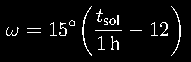
\includegraphics[width=34.5479mm,height=11.2500mm,keepaspectratio]{../figuras/EQ_horario.pdf}};
\node[anchor=north west,inner sep=0pt,text width=59.37500mm,align=left,text=ink,font=\fontsize{10.6299}{11.4803}\selectfont ] at ([xshift=86.87500mm,yshift=-65.00000mm]current page.north west) {Manhã: ω < 0°\\Tarde: ω > 0°};
\node[anchor=north west,inner sep=0pt,text width=141.25000mm,align=left,text=yel,font=\fontsize{9.2126}{9.9496}\selectfont ] at ([xshift=9.37500mm,yshift=-76.25000mm]current page.north west) {Ângulos em graus na exposição; conversão para radianos no código.};
\node[anchor=north west,inner sep=0pt,text width=145.00000mm,align=left,text=ink,font=\fontsize{6.0236}{6.5055}\selectfont ] at ([xshift=7.50000mm,yshift=-81.62500mm]current page.north west) {Fontes: Duffie, Beckman e Blair (2020), p. 13–15; Reda e Andreas (2008), p. 10–11.};
\draw[yel,line width=.10mm] ([xshift=6mm,yshift=-84.48mm]current page.north west)--([xshift=153.84mm,yshift=-84.48mm]current page.north west);
\node[anchor=north west,inner sep=0pt,text width=138.62500mm,align=left,text=ink,font=\fontsize{5.6693}{6.1228}\selectfont ] at ([xshift=6.96000mm,yshift=-86.37500mm]current page.north west) {Recurso solar e modelagem da conversão fotovoltaica};
\node[anchor=north west,inner sep=0pt,text width=6.25000mm,align=left,text=yel,font=\fontsize{7.0866}{7.6535}\selectfont \bfseries ] at ([xshift=147.50000mm,yshift=-86.12500mm]current page.north west) {2};
\end{tikzpicture}
\end{frame}
\begin{frame}[plain]
\begin{tikzpicture}[remember picture,overlay]
\node[anchor=north west,inner sep=0pt,text width=60.00000mm,align=left,text=ink,font=\fontsize{7.0866}{7.6535}\selectfont \bfseries ] at ([xshift=6.96000mm,yshift=-1.25000mm]current page.north west) {UFPB  ·  CEAR  ·  PPGER};
\node[anchor=north west,inner sep=0pt,text width=38.75000mm,align=left,text=ink,font=\fontsize{7.0866}{7.6535}\selectfont ] at ([xshift=114.00000mm,yshift=-1.25000mm]current page.north west) {SPGER0046  ·  03 DEZ 2026};
\draw[yel,line width=.12mm] ([xshift=6mm,yshift=-4.56mm]current page.north west)--([xshift=153.84mm,yshift=-4.56mm]current page.north west);
\node[anchor=north west,inner sep=0pt,text width=145.62500mm,align=left,text=ink,font=\fontsize{14.5275}{15.6897}\selectfont \bfseries ] at ([xshift=6.96000mm,yshift=-7.62500mm]current page.north west) {1.1 · IRRADIÂNCIA EXTRATERRESTRE};
\node[anchor=north west,inner sep=0pt,text width=143.75000mm,align=left,text=yel,font=\fontsize{10.2756}{11.0976}\selectfont ] at ([xshift=7.44000mm,yshift=-17.50000mm]current page.north west) {Referência radiativa anterior à interação com a atmosfera.};
\node[anchor=north west,inner sep=0pt] at ([xshift=30.6191mm,yshift=-24.3750mm]current page.north west) {
\includegraphics[width=42.5119mm,height=9.3750mm,keepaspectratio]{../figuras/EQ_distancia.pdf}};
\node[anchor=north west,inner sep=0pt,text width=48.75000mm,align=left,text=ink,font=\fontsize{9.9212}{10.7149}\selectfont ] at ([xshift=102.50000mm,yshift=-23.75000mm]current page.north west) {Gsc = 1 366,1 W m$^{-2}$\\Valor fixado no pvlib do projeto.};
\node[anchor=north west,inner sep=0pt] at ([xshift=34.8337mm,yshift=-37.5000mm]current page.north west) {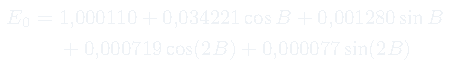
\includegraphics[width=90.3326mm,height=13.7500mm,keepaspectratio]{../figuras/EQ_spencer.pdf}};
\node[anchor=north west,inner sep=0pt,text width=136.25000mm,align=left,text=yel,font=\fontsize{9.9212}{10.7149}\selectfont ] at ([xshift=12.50000mm,yshift=-53.75000mm]current page.north west) {B = 2π(n − 1)/365; n = dia do ano; B em radianos.};
\node[anchor=north west,inner sep=0pt] at ([xshift=50.6144mm,yshift=-62.5000mm]current page.north west) {
\includegraphics[width=58.7712mm,height=8.1250mm,keepaspectratio]{../figuras/EQ_projecao.pdf}};
\node[anchor=north west,inner sep=0pt,text width=142.50000mm,align=left,text=yel,font=\fontsize{10.2756}{11.0976}\selectfont ] at ([xshift=8.75000mm,yshift=-75.00000mm]current page.north west) {$G_{0h}$ é referência extraterrestre; GHI é irradiância na superfície.};
\node[anchor=north west,inner sep=0pt,text width=145.00000mm,align=left,text=ink,font=\fontsize{6.0236}{6.5055}\selectfont ] at ([xshift=7.50000mm,yshift=-81.62500mm]current page.north west) {Fontes: Duffie, Beckman e Blair (2020), p. 9; pvlib 0.16.1, get\_extra\_radiation.};
\draw[yel,line width=.10mm] ([xshift=6mm,yshift=-84.48mm]current page.north west)--([xshift=153.84mm,yshift=-84.48mm]current page.north west);
\node[anchor=north west,inner sep=0pt,text width=138.62500mm,align=left,text=ink,font=\fontsize{5.6693}{6.1228}\selectfont ] at ([xshift=6.96000mm,yshift=-86.37500mm]current page.north west) {Recurso solar e modelagem da conversão fotovoltaica};
\node[anchor=north west,inner sep=0pt,text width=6.25000mm,align=left,text=yel,font=\fontsize{7.0866}{7.6535}\selectfont \bfseries ] at ([xshift=147.50000mm,yshift=-86.12500mm]current page.north west) {3};
\end{tikzpicture}
\end{frame}
\begin{frame}[plain]
\begin{tikzpicture}[remember picture,overlay]
\node[anchor=north west,inner sep=0pt,text width=60.00000mm,align=left,text=ink,font=\fontsize{7.0866}{7.6535}\selectfont \bfseries ] at ([xshift=6.96000mm,yshift=-1.25000mm]current page.north west) {UFPB  ·  CEAR  ·  PPGER};
\node[anchor=north west,inner sep=0pt,text width=38.75000mm,align=left,text=ink,font=\fontsize{7.0866}{7.6535}\selectfont ] at ([xshift=114.00000mm,yshift=-1.25000mm]current page.north west) {SPGER0046  ·  03 DEZ 2026};
\draw[yel,line width=.12mm] ([xshift=6mm,yshift=-4.56mm]current page.north west)--([xshift=153.84mm,yshift=-4.56mm]current page.north west);
\node[anchor=north west,inner sep=0pt,text width=145.62500mm,align=left,text=ink,font=\fontsize{14.5275}{15.6897}\selectfont \bfseries ] at ([xshift=6.96000mm,yshift=-7.62500mm]current page.north west) {1.1 · IMPLEMENTAÇÃO COMPUTACIONAL};
\node[anchor=north west,inner sep=0pt,text width=143.75000mm,align=left,text=yel,font=\fontsize{10.2756}{11.0976}\selectfont ] at ([xshift=7.44000mm,yshift=-17.50000mm]current page.north west) {SPA e Spencer recebem entradas temporais e cumprem funções distintas.};
\node[anchor=north west,inner sep=0pt] at ([xshift=20.9043mm,yshift=-25.0000mm]current page.north west) {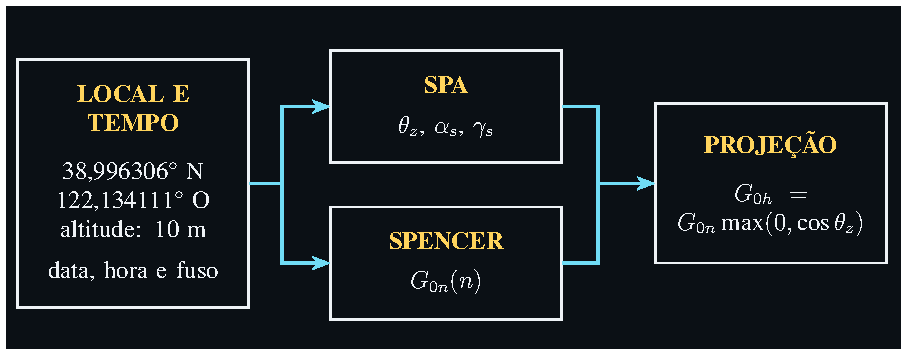
\includegraphics[width=118.1914mm,height=46.2500mm,keepaspectratio]{../figuras/D02_fluxo_geometria.pdf}};
\node[anchor=north west,inner sep=0pt,text width=142.50000mm,align=left,text=yel,font=\fontsize{10.2756}{11.0976}\selectfont ] at ([xshift=10.00000mm,yshift=-71.87500mm]current page.north west) {Rótulo = início · Δt = 15 min · cálculo em t + 7 min 30 s};
\node[anchor=north west,inner sep=0pt,text width=142.50000mm,align=left,text=ink,font=\fontsize{9.9212}{10.7149}\selectfont ] at ([xshift=10.00000mm,yshift=-77.50000mm]current page.north west) {Em 17/05/2024: America/Los\_Angeles = UTC−7.};
\node[anchor=north west,inner sep=0pt,text width=145.00000mm,align=left,text=ink,font=\fontsize{6.0236}{6.5055}\selectfont ] at ([xshift=7.50000mm,yshift=-81.62500mm]current page.north west) {Fontes: configuração do projeto PVDAQ 2107; Reda e Andreas (2008); pvlib 0.16.1.};
\draw[yel,line width=.10mm] ([xshift=6mm,yshift=-84.48mm]current page.north west)--([xshift=153.84mm,yshift=-84.48mm]current page.north west);
\node[anchor=north west,inner sep=0pt,text width=138.62500mm,align=left,text=ink,font=\fontsize{5.6693}{6.1228}\selectfont ] at ([xshift=6.96000mm,yshift=-86.37500mm]current page.north west) {Recurso solar e modelagem da conversão fotovoltaica};
\node[anchor=north west,inner sep=0pt,text width=6.25000mm,align=left,text=yel,font=\fontsize{7.0866}{7.6535}\selectfont \bfseries ] at ([xshift=147.50000mm,yshift=-86.12500mm]current page.north west) {4};
\end{tikzpicture}
\end{frame}
\begin{frame}[plain]
\begin{tikzpicture}[remember picture,overlay]
\node[anchor=north west,inner sep=0pt,text width=60.00000mm,align=left,text=ink,font=\fontsize{7.0866}{7.6535}\selectfont \bfseries ] at ([xshift=6.96000mm,yshift=-1.25000mm]current page.north west) {UFPB  ·  CEAR  ·  PPGER};
\node[anchor=north west,inner sep=0pt,text width=38.75000mm,align=left,text=ink,font=\fontsize{7.0866}{7.6535}\selectfont ] at ([xshift=114.00000mm,yshift=-1.25000mm]current page.north west) {SPGER0046  ·  03 DEZ 2026};
\draw[yel,line width=.12mm] ([xshift=6mm,yshift=-4.56mm]current page.north west)--([xshift=153.84mm,yshift=-4.56mm]current page.north west);
\node[anchor=north west,inner sep=0pt,text width=145.62500mm,align=left,text=ink,font=\fontsize{14.5275}{15.6897}\selectfont \bfseries ] at ([xshift=6.96000mm,yshift=-7.62500mm]current page.north west) {1.1 · PVDAQ 2107 EM 17/05/2024};
\node[anchor=north west,inner sep=0pt,text width=143.75000mm,align=left,text=yel,font=\fontsize{10.2756}{11.0976}\selectfont ] at ([xshift=7.44000mm,yshift=-17.50000mm]current page.north west) {Arbuckle, Califórnia · 38,996306° N; 122,134111° O · 10 m};
\node[anchor=north west,inner sep=0pt] at ([xshift=6.2500mm,yshift=-24.3862mm]current page.north west) {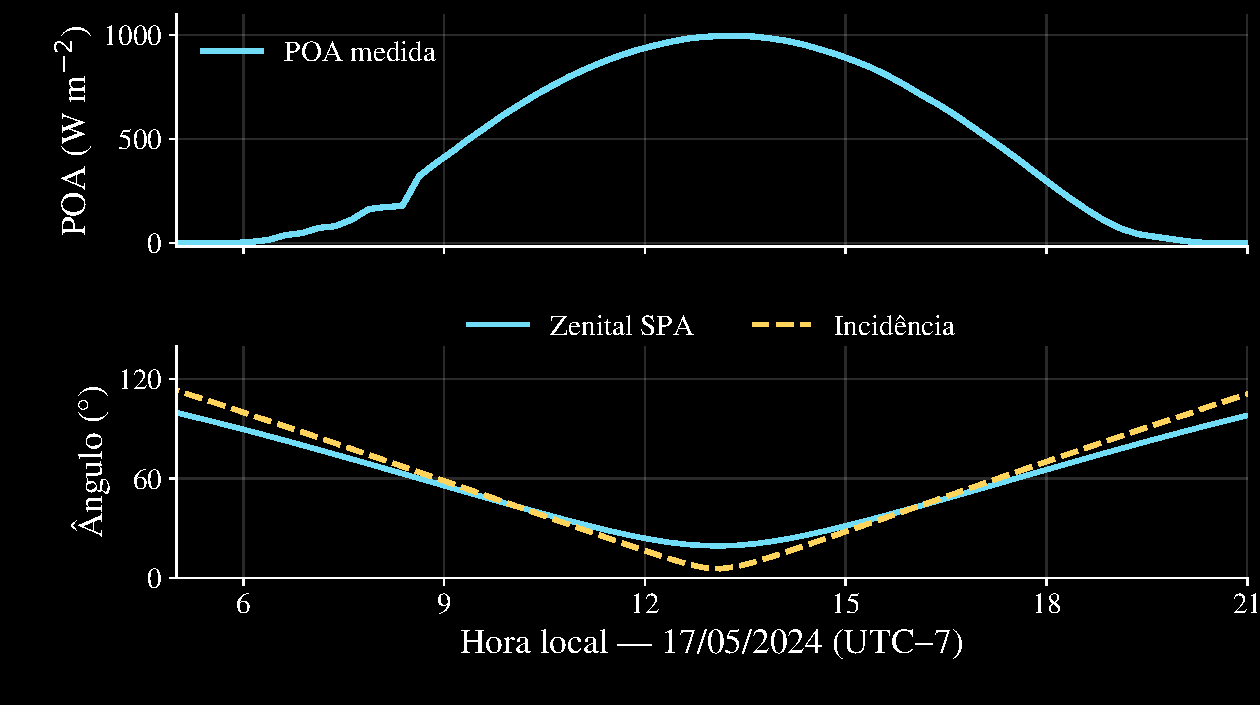
\includegraphics[width=99.3750mm,height=55.6027mm,keepaspectratio]{../figuras/G01_recurso_geometria_escuro.pdf}};
\node[anchor=north west,inner sep=0pt,text width=41.87500mm,align=left,text=yel,font=\fontsize{11.6929}{12.6283}\selectfont \bfseries ] at ([xshift=110.62500mm,yshift=-28.12500mm]current page.north west) {POA medida};
\node[anchor=north west,inner sep=0pt,text width=41.87500mm,align=left,text=ink,font=\fontsize{10.6299}{11.4803}\selectfont ] at ([xshift=110.62500mm,yshift=-34.37500mm]current page.north west) {Média em intervalos\\de 15 minutos.};
\node[anchor=north west,inner sep=0pt,text width=41.87500mm,align=left,text=yel,font=\fontsize{11.6929}{12.6283}\selectfont \bfseries ] at ([xshift=110.62500mm,yshift=-48.12500mm]current page.north west) {Ângulos calculados};
\node[anchor=north west,inner sep=0pt,text width=41.87500mm,align=left,text=ink,font=\fontsize{10.6299}{11.4803}\selectfont ] at ([xshift=110.62500mm,yshift=-54.37500mm]current page.north west) {SPA e orientação\\do arranjo.};
\node[anchor=north west,inner sep=0pt,text width=41.87500mm,align=left,text=ink,font=\fontsize{10.6299}{11.4803}\selectfont ] at ([xshift=110.62500mm,yshift=-68.12500mm]current page.north west) {Inclinação: 25°\\Azimute: 180°};
\node[anchor=north west,inner sep=0pt,text width=145.00000mm,align=left,text=ink,font=\fontsize{6.0236}{6.5055}\selectfont ] at ([xshift=7.50000mm,yshift=-81.62500mm]current page.north west) {G01 — Fonte: POA/PVDAQ 2107 e cálculos SPA da equipe. Curvas no ponto médio; sem interpolação.};
\draw[yel,line width=.10mm] ([xshift=6mm,yshift=-84.48mm]current page.north west)--([xshift=153.84mm,yshift=-84.48mm]current page.north west);
\node[anchor=north west,inner sep=0pt,text width=138.62500mm,align=left,text=ink,font=\fontsize{5.6693}{6.1228}\selectfont ] at ([xshift=6.96000mm,yshift=-86.37500mm]current page.north west) {Recurso solar e modelagem da conversão fotovoltaica};
\node[anchor=north west,inner sep=0pt,text width=6.25000mm,align=left,text=yel,font=\fontsize{7.0866}{7.6535}\selectfont \bfseries ] at ([xshift=147.50000mm,yshift=-86.12500mm]current page.north west) {5};
\end{tikzpicture}
\end{frame}
\begin{frame}[plain]
\begin{tikzpicture}[remember picture,overlay]
\node[anchor=north west,inner sep=0pt,text width=60.00000mm,align=left,text=ink,font=\fontsize{7.0866}{7.6535}\selectfont \bfseries ] at ([xshift=6.96000mm,yshift=-1.25000mm]current page.north west) {UFPB  ·  CEAR  ·  PPGER};
\node[anchor=north west,inner sep=0pt,text width=38.75000mm,align=left,text=ink,font=\fontsize{7.0866}{7.6535}\selectfont ] at ([xshift=114.00000mm,yshift=-1.25000mm]current page.north west) {SPGER0046  ·  03 DEZ 2026};
\draw[yel,line width=.12mm] ([xshift=6mm,yshift=-4.56mm]current page.north west)--([xshift=153.84mm,yshift=-4.56mm]current page.north west);
\node[anchor=north west,inner sep=0pt,text width=145.62500mm,align=left,text=ink,font=\fontsize{14.5275}{15.6897}\selectfont \bfseries ] at ([xshift=6.96000mm,yshift=-7.62500mm]current page.north west) {1.1 · SÍNTESE E LIMITES};
\node[anchor=north west,inner sep=0pt,text width=143.75000mm,align=left,text=yel,font=\fontsize{10.2756}{11.0976}\selectfont ] at ([xshift=7.44000mm,yshift=-17.50000mm]current page.north west) {A geometria estabelece o referencial para caracterizar o recurso solar.};
\node[anchor=north west,inner sep=0pt,text width=141.25000mm,align=left,text=yel,font=\fontsize{12.0472}{13.0110}\selectfont \bfseries ] at ([xshift=9.37500mm,yshift=-26.25000mm]current page.north west) {A GEOMETRIA FORNECE};
\node[anchor=north west,inner sep=0pt,text width=141.25000mm,align=left,text=ink,font=\fontsize{11.3386}{12.2456}\selectfont ] at ([xshift=9.37500mm,yshift=-33.12500mm]current page.north west) {Direção solar, duração do dia e fator de projeção do feixe.};
\node[anchor=north west,inner sep=0pt,text width=141.25000mm,align=left,text=yel,font=\fontsize{12.0472}{13.0110}\selectfont \bfseries ] at ([xshift=9.37500mm,yshift=-43.75000mm]current page.north west) {A ATMOSFERA MODIFICA};
\node[anchor=north west,inner sep=0pt,text width=141.25000mm,align=left,text=ink,font=\fontsize{11.3386}{12.2456}\selectfont ] at ([xshift=9.37500mm,yshift=-50.62500mm]current page.north west) {Transmissão, absorção e espalhamento da radiação.};
\node[anchor=north west,inner sep=0pt,text width=141.25000mm,align=left,text=yel,font=\fontsize{12.0472}{13.0110}\selectfont \bfseries ] at ([xshift=9.37500mm,yshift=-61.25000mm]current page.north west) {A OBSERVAÇÃO PERMITE CONFRONTAR};
\node[anchor=north west,inner sep=0pt,text width=141.25000mm,align=left,text=ink,font=\fontsize{11.3386}{12.2456}\selectfont ] at ([xshift=9.37500mm,yshift=-68.12500mm]current page.north west) {Irradiância no plano do sensor e evolução temporal medida.};
\node[anchor=north west,inner sep=0pt,text width=141.25000mm,align=left,text=yel,font=\fontsize{9.5669}{10.3323}\selectfont ] at ([xshift=9.37500mm,yshift=-76.87500mm]current page.north west) {1.2 — Irradiância e irradiação; componentes GHI, DNI, DHI e POA.};
\node[anchor=north west,inner sep=0pt,text width=145.00000mm,align=left,text=ink,font=\fontsize{6.0236}{6.5055}\selectfont ] at ([xshift=7.50000mm,yshift=-81.62500mm]current page.north west) {Fontes: Duffie, Beckman e Blair (2020), p. 9–15; Sengupta et al. (2024), cap. 2, p. 5–10.};
\draw[yel,line width=.10mm] ([xshift=6mm,yshift=-84.48mm]current page.north west)--([xshift=153.84mm,yshift=-84.48mm]current page.north west);
\node[anchor=north west,inner sep=0pt,text width=138.62500mm,align=left,text=ink,font=\fontsize{5.6693}{6.1228}\selectfont ] at ([xshift=6.96000mm,yshift=-86.37500mm]current page.north west) {Recurso solar e modelagem da conversão fotovoltaica};
\node[anchor=north west,inner sep=0pt,text width=6.25000mm,align=left,text=yel,font=\fontsize{7.0866}{7.6535}\selectfont \bfseries ] at ([xshift=147.50000mm,yshift=-86.12500mm]current page.north west) {6};
\end{tikzpicture}
\end{frame}
\begin{frame}[plain]
\begin{tikzpicture}[remember picture,overlay]
\node[anchor=north west,inner sep=0pt,text width=60.00000mm,align=left,text=ink,font=\fontsize{7.0866}{7.6535}\selectfont \bfseries ] at ([xshift=6.96000mm,yshift=-1.25000mm]current page.north west) {UFPB  ·  CEAR  ·  PPGER};
\node[anchor=north west,inner sep=0pt,text width=38.75000mm,align=left,text=ink,font=\fontsize{7.0866}{7.6535}\selectfont ] at ([xshift=114.00000mm,yshift=-1.25000mm]current page.north west) {SPGER0046  ·  03 DEZ 2026};
\draw[yel,line width=.12mm] ([xshift=6mm,yshift=-4.56mm]current page.north west)--([xshift=153.84mm,yshift=-4.56mm]current page.north west);
\node[anchor=north west,inner sep=0pt,text width=145.62500mm,align=left,text=ink,font=\fontsize{14.5275}{15.6897}\selectfont \bfseries ] at ([xshift=6.96000mm,yshift=-7.62500mm]current page.north west) {1.2 · IRRADIÂNCIA E IRRADIAÇÃO};
\node[anchor=north west,inner sep=0pt,text width=143.75000mm,align=left,text=yel,font=\fontsize{10.2756}{11.0976}\selectfont ] at ([xshift=7.44000mm,yshift=-17.50000mm]current page.north west) {A irradiância é potência por área; a irradiação é energia por área.};
\node[anchor=north west,inner sep=0pt] at ([xshift=57.7905mm,yshift=-27.5000mm]current page.north west) {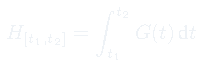
\includegraphics[width=44.4189mm,height=14.3750mm,keepaspectratio]{../figuras/EQ_integracao.pdf}};
\node[anchor=north west,inner sep=0pt,text width=63.75000mm,align=left,text=yel,font=\fontsize{12.4015}{13.3937}\selectfont \bfseries ] at ([xshift=9.37500mm,yshift=-48.12500mm]current page.north west) {IRRADIÂNCIA G};
\node[anchor=north west,inner sep=0pt,text width=63.75000mm,align=left,text=ink,font=\fontsize{11.3386}{12.2456}\selectfont ] at ([xshift=9.37500mm,yshift=-55.62500mm]current page.north west) {W/m²\\Plano e suporte temporal definidos.};
\node[anchor=north west,inner sep=0pt,text width=63.75000mm,align=left,text=yel,font=\fontsize{12.4015}{13.3937}\selectfont \bfseries ] at ([xshift=89.37500mm,yshift=-48.12500mm]current page.north west) {IRRADIAÇÃO H};
\node[anchor=north west,inner sep=0pt,text width=63.75000mm,align=left,text=ink,font=\fontsize{11.3386}{12.2456}\selectfont ] at ([xshift=89.37500mm,yshift=-55.62500mm]current page.north west) {J/m², Wh/m² ou kWh/m²\\Intervalo de integração declarado.};
\node[anchor=north west,inner sep=0pt,text width=140.00000mm,align=left,text=yel,font=\fontsize{9.9212}{10.7149}\selectfont ] at ([xshift=9.37500mm,yshift=-73.75000mm]current page.north west) {Médias de intervalo: somar G médio × duração, somente nos intervalos válidos.};
\node[anchor=north west,inner sep=0pt,text width=145.00000mm,align=left,text=ink,font=\fontsize{6.0236}{6.5055}\selectfont ] at ([xshift=7.50000mm,yshift=-81.62500mm]current page.north west) {Fonte: Duffie, Beckman e Blair (2020), p. 10.};
\draw[yel,line width=.10mm] ([xshift=6mm,yshift=-84.48mm]current page.north west)--([xshift=153.84mm,yshift=-84.48mm]current page.north west);
\node[anchor=north west,inner sep=0pt,text width=138.62500mm,align=left,text=ink,font=\fontsize{5.6693}{6.1228}\selectfont ] at ([xshift=6.96000mm,yshift=-86.37500mm]current page.north west) {Recurso solar e modelagem da conversão fotovoltaica};
\node[anchor=north west,inner sep=0pt,text width=6.25000mm,align=left,text=yel,font=\fontsize{7.0866}{7.6535}\selectfont \bfseries ] at ([xshift=147.50000mm,yshift=-86.12500mm]current page.north west) {7};
\end{tikzpicture}
\end{frame}
\begin{frame}[plain]
\begin{tikzpicture}[remember picture,overlay]
\node[anchor=north west,inner sep=0pt,text width=60.00000mm,align=left,text=ink,font=\fontsize{7.0866}{7.6535}\selectfont \bfseries ] at ([xshift=6.96000mm,yshift=-1.25000mm]current page.north west) {UFPB  ·  CEAR  ·  PPGER};
\node[anchor=north west,inner sep=0pt,text width=38.75000mm,align=left,text=ink,font=\fontsize{7.0866}{7.6535}\selectfont ] at ([xshift=114.00000mm,yshift=-1.25000mm]current page.north west) {SPGER0046  ·  03 DEZ 2026};
\draw[yel,line width=.12mm] ([xshift=6mm,yshift=-4.56mm]current page.north west)--([xshift=153.84mm,yshift=-4.56mm]current page.north west);
\node[anchor=north west,inner sep=0pt,text width=145.62500mm,align=left,text=ink,font=\fontsize{14.5275}{15.6897}\selectfont \bfseries ] at ([xshift=6.96000mm,yshift=-7.62500mm]current page.north west) {1.2 · COMPONENTES DA RADIAÇÃO};
\node[anchor=north west,inner sep=0pt,text width=143.75000mm,align=left,text=yel,font=\fontsize{10.2756}{11.0976}\selectfont ] at ([xshift=7.44000mm,yshift=-17.50000mm]current page.north west) {A unidade é comum; a direção e o plano de recepção são diferentes.};
\node[anchor=north west,inner sep=0pt] at ([xshift=41.6331mm,yshift=-28.7500mm]current page.north west) {
\includegraphics[width=76.7338mm,height=10.0000mm,keepaspectratio]{../figuras/EQ_fechamento.pdf}};
\node[anchor=north west,inner sep=0pt,text width=26.25000mm,align=left,text=yel,font=\fontsize{12.4015}{13.3937}\selectfont \bfseries ] at ([xshift=9.37500mm,yshift=-47.50000mm]current page.north west) {DNI};
\node[anchor=north west,inner sep=0pt,text width=106.25000mm,align=left,text=ink,font=\fontsize{11.3386}{12.2456}\selectfont ] at ([xshift=37.50000mm,yshift=-47.50000mm]current page.north west) {Direta normal à direção solar.};
\node[anchor=north west,inner sep=0pt,text width=26.25000mm,align=left,text=yel,font=\fontsize{12.4015}{13.3937}\selectfont \bfseries ] at ([xshift=9.37500mm,yshift=-56.25000mm]current page.north west) {DHI};
\node[anchor=north west,inner sep=0pt,text width=106.25000mm,align=left,text=ink,font=\fontsize{11.3386}{12.2456}\selectfont ] at ([xshift=37.50000mm,yshift=-56.25000mm]current page.north west) {Difusa recebida na horizontal.};
\node[anchor=north west,inner sep=0pt,text width=26.25000mm,align=left,text=yel,font=\fontsize{12.4015}{13.3937}\selectfont \bfseries ] at ([xshift=9.37500mm,yshift=-65.00000mm]current page.north west) {GHI};
\node[anchor=north west,inner sep=0pt,text width=106.25000mm,align=left,text=ink,font=\fontsize{11.3386}{12.2456}\selectfont ] at ([xshift=37.50000mm,yshift=-65.00000mm]current page.north west) {Global recebida na horizontal.};
\node[anchor=north west,inner sep=0pt,text width=26.25000mm,align=left,text=yel,font=\fontsize{12.4015}{13.3937}\selectfont \bfseries ] at ([xshift=9.37500mm,yshift=-73.75000mm]current page.north west) {POA};
\node[anchor=north west,inner sep=0pt,text width=106.25000mm,align=left,text=ink,font=\fontsize{11.3386}{12.2456}\selectfont ] at ([xshift=37.50000mm,yshift=-73.75000mm]current page.north west) {Irradiância no plano do arranjo.};
\node[anchor=north west,inner sep=0pt,text width=145.00000mm,align=left,text=ink,font=\fontsize{6.0236}{6.5055}\selectfont ] at ([xshift=7.50000mm,yshift=-81.62500mm]current page.north west) {Fonte: Sengupta et al. (2024), cap. 2, p. 9–10; cap. 3, p. 5.};
\draw[yel,line width=.10mm] ([xshift=6mm,yshift=-84.48mm]current page.north west)--([xshift=153.84mm,yshift=-84.48mm]current page.north west);
\node[anchor=north west,inner sep=0pt,text width=138.62500mm,align=left,text=ink,font=\fontsize{5.6693}{6.1228}\selectfont ] at ([xshift=6.96000mm,yshift=-86.37500mm]current page.north west) {Recurso solar e modelagem da conversão fotovoltaica};
\node[anchor=north west,inner sep=0pt,text width=6.25000mm,align=left,text=yel,font=\fontsize{7.0866}{7.6535}\selectfont \bfseries ] at ([xshift=147.50000mm,yshift=-86.12500mm]current page.north west) {8};
\end{tikzpicture}
\end{frame}
\begin{frame}[plain]
\begin{tikzpicture}[remember picture,overlay]
\node[anchor=north west,inner sep=0pt,text width=60.00000mm,align=left,text=ink,font=\fontsize{7.0866}{7.6535}\selectfont \bfseries ] at ([xshift=6.96000mm,yshift=-1.25000mm]current page.north west) {UFPB  ·  CEAR  ·  PPGER};
\node[anchor=north west,inner sep=0pt,text width=38.75000mm,align=left,text=ink,font=\fontsize{7.0866}{7.6535}\selectfont ] at ([xshift=114.00000mm,yshift=-1.25000mm]current page.north west) {SPGER0046  ·  03 DEZ 2026};
\draw[yel,line width=.12mm] ([xshift=6mm,yshift=-4.56mm]current page.north west)--([xshift=153.84mm,yshift=-4.56mm]current page.north west);
\node[anchor=north west,inner sep=0pt,text width=145.62500mm,align=left,text=ink,font=\fontsize{14.5275}{15.6897}\selectfont \bfseries ] at ([xshift=6.96000mm,yshift=-7.62500mm]current page.north west) {1.3 · MODULAÇÃO ATMOSFÉRICA};
\node[anchor=north west,inner sep=0pt,text width=143.75000mm,align=left,text=yel,font=\fontsize{10.2756}{11.0976}\selectfont ] at ([xshift=7.44000mm,yshift=-17.50000mm]current page.north west) {Absorção e espalhamento modificam o campo radiativo.};
\node[anchor=north west,inner sep=0pt,text width=42.50000mm,align=left,text=yel,font=\fontsize{12.4015}{13.3937}\selectfont \bfseries ] at ([xshift=9.37500mm,yshift=-29.37500mm]current page.north west) {NUVENS};
\node[anchor=north west,inner sep=0pt,text width=42.50000mm,align=left,text=ink,font=\fontsize{11.3386}{12.2456}\selectfont ] at ([xshift=9.37500mm,yshift=-38.75000mm]current page.north west) {Obstrução do feixe.\\Redistribuição difusa.\\Variações rápidas.};
\node[anchor=north west,inner sep=0pt,text width=42.50000mm,align=left,text=yel,font=\fontsize{12.4015}{13.3937}\selectfont \bfseries ] at ([xshift=58.75000mm,yshift=-29.37500mm]current page.north west) {AEROSSÓIS};
\node[anchor=north west,inner sep=0pt,text width=42.50000mm,align=left,text=ink,font=\fontsize{11.3386}{12.2456}\selectfont ] at ([xshift=58.75000mm,yshift=-38.75000mm]current page.north west) {Profundidade óptica.\\Absorção e\\espalhamento.};
\node[anchor=north west,inner sep=0pt,text width=43.75000mm,align=left,text=yel,font=\fontsize{12.4015}{13.3937}\selectfont \bfseries ] at ([xshift=108.12500mm,yshift=-29.37500mm]current page.north west) {VAPOR DE ÁGUA};
\node[anchor=north west,inner sep=0pt,text width=43.75000mm,align=left,text=ink,font=\fontsize{11.3386}{12.2456}\selectfont ] at ([xshift=108.12500mm,yshift=-38.75000mm]current page.north west) {Absorção espectral.\\Quantidade integrada\\na coluna.};
\node[anchor=north west,inner sep=0pt,text width=141.25000mm,align=left,text=yel,font=\fontsize{10.9842}{11.8630}\selectfont ] at ([xshift=9.37500mm,yshift=-71.87500mm]current page.north west) {POA isolada não permite separar quantitativamente esses mecanismos.};
\node[anchor=north west,inner sep=0pt,text width=145.00000mm,align=left,text=ink,font=\fontsize{6.0236}{6.5055}\selectfont ] at ([xshift=7.50000mm,yshift=-81.62500mm]current page.north west) {Fonte: Sengupta et al. (2024), cap. 2, p. 6–7; cap. 5, p. 10.};
\draw[yel,line width=.10mm] ([xshift=6mm,yshift=-84.48mm]current page.north west)--([xshift=153.84mm,yshift=-84.48mm]current page.north west);
\node[anchor=north west,inner sep=0pt,text width=138.62500mm,align=left,text=ink,font=\fontsize{5.6693}{6.1228}\selectfont ] at ([xshift=6.96000mm,yshift=-86.37500mm]current page.north west) {Recurso solar e modelagem da conversão fotovoltaica};
\node[anchor=north west,inner sep=0pt,text width=6.25000mm,align=left,text=yel,font=\fontsize{7.0866}{7.6535}\selectfont \bfseries ] at ([xshift=147.50000mm,yshift=-86.12500mm]current page.north west) {9};
\end{tikzpicture}
\end{frame}
\begin{frame}[plain]
\begin{tikzpicture}[remember picture,overlay]
\node[anchor=north west,inner sep=0pt,text width=60.00000mm,align=left,text=ink,font=\fontsize{7.0866}{7.6535}\selectfont \bfseries ] at ([xshift=6.96000mm,yshift=-1.25000mm]current page.north west) {UFPB  ·  CEAR  ·  PPGER};
\node[anchor=north west,inner sep=0pt,text width=38.75000mm,align=left,text=ink,font=\fontsize{7.0866}{7.6535}\selectfont ] at ([xshift=114.00000mm,yshift=-1.25000mm]current page.north west) {SPGER0046  ·  03 DEZ 2026};
\draw[yel,line width=.12mm] ([xshift=6mm,yshift=-4.56mm]current page.north west)--([xshift=153.84mm,yshift=-4.56mm]current page.north west);
\node[anchor=north west,inner sep=0pt,text width=145.62500mm,align=left,text=ink,font=\fontsize{14.5275}{15.6897}\selectfont \bfseries ] at ([xshift=6.96000mm,yshift=-7.62500mm]current page.north west) {1.3 · VARIABILIDADE E ESCALAS};
\node[anchor=north west,inner sep=0pt,text width=143.75000mm,align=left,text=yel,font=\fontsize{10.2756}{11.0976}\selectfont ] at ([xshift=7.44000mm,yshift=-17.50000mm]current page.north west) {A componente, o intervalo e o domínio espacial definem a análise.};
\node[anchor=north west,inner sep=0pt,text width=140.00000mm,align=left,text=yel,font=\fontsize{12.4015}{13.3937}\selectfont \bfseries ] at ([xshift=9.37500mm,yshift=-27.50000mm]current page.north west) {NO TEMPO};
\node[anchor=north west,inner sep=0pt,text width=140.00000mm,align=left,text=ink,font=\fontsize{11.3386}{12.2456}\selectfont ] at ([xshift=9.37500mm,yshift=-35.00000mm]current page.north west) {Ciclo diário, sazonalidade e variações meteorológicas.};
\node[anchor=north west,inner sep=0pt,text width=140.00000mm,align=left,text=yel,font=\fontsize{12.4015}{13.3937}\selectfont \bfseries ] at ([xshift=9.37500mm,yshift=-46.25000mm]current page.north west) {NO ESPAÇO};
\node[anchor=north west,inner sep=0pt,text width=140.00000mm,align=left,text=ink,font=\fontsize{11.3386}{12.2456}\selectfont ] at ([xshift=9.37500mm,yshift=-53.75000mm]current page.north west) {Nuvens e relevo limitam a extrapolação entre localidades.};
\node[anchor=north west,inner sep=0pt,text width=140.00000mm,align=left,text=yel,font=\fontsize{12.4015}{13.3937}\selectfont \bfseries ] at ([xshift=9.37500mm,yshift=-65.00000mm]current page.north west) {NA RESOLUÇÃO};
\node[anchor=north west,inner sep=0pt,text width=140.00000mm,align=left,text=ink,font=\fontsize{10.9842}{11.8630}\selectfont ] at ([xshift=9.37500mm,yshift=-72.50000mm]current page.north west) {Médias temporais suavizam flutuações; um dia não estabelece climatologia.};
\node[anchor=north west,inner sep=0pt,text width=145.00000mm,align=left,text=ink,font=\fontsize{6.0236}{6.5055}\selectfont ] at ([xshift=7.50000mm,yshift=-81.62500mm]current page.north west) {Fonte: Sengupta et al. (2024), cap. 6, p. 1–2, 17 e 24–25.};
\draw[yel,line width=.10mm] ([xshift=6mm,yshift=-84.48mm]current page.north west)--([xshift=153.84mm,yshift=-84.48mm]current page.north west);
\node[anchor=north west,inner sep=0pt,text width=138.62500mm,align=left,text=ink,font=\fontsize{5.6693}{6.1228}\selectfont ] at ([xshift=6.96000mm,yshift=-86.37500mm]current page.north west) {Recurso solar e modelagem da conversão fotovoltaica};
\node[anchor=north west,inner sep=0pt,text width=6.25000mm,align=left,text=yel,font=\fontsize{7.0866}{7.6535}\selectfont \bfseries ] at ([xshift=147.50000mm,yshift=-86.12500mm]current page.north west) {10};
\end{tikzpicture}
\end{frame}
\begin{frame}[plain]
\begin{tikzpicture}[remember picture,overlay]
\node[anchor=north west,inner sep=0pt,text width=60.00000mm,align=left,text=ink,font=\fontsize{7.0866}{7.6535}\selectfont \bfseries ] at ([xshift=6.96000mm,yshift=-1.25000mm]current page.north west) {UFPB  ·  CEAR  ·  PPGER};
\node[anchor=north west,inner sep=0pt,text width=38.75000mm,align=left,text=ink,font=\fontsize{7.0866}{7.6535}\selectfont ] at ([xshift=114.00000mm,yshift=-1.25000mm]current page.north west) {SPGER0046  ·  03 DEZ 2026};
\draw[yel,line width=.12mm] ([xshift=6mm,yshift=-4.56mm]current page.north west)--([xshift=153.84mm,yshift=-4.56mm]current page.north west);
\node[anchor=north west,inner sep=0pt,text width=145.62500mm,align=left,text=ink,font=\fontsize{14.5275}{15.6897}\selectfont \bfseries ] at ([xshift=6.96000mm,yshift=-7.62500mm]current page.north west) {1.4 · MEDIÇÃO E ESTIMATIVA};
\node[anchor=north west,inner sep=0pt,text width=143.75000mm,align=left,text=yel,font=\fontsize{10.2756}{11.0976}\selectfont ] at ([xshift=7.44000mm,yshift=-17.50000mm]current page.north west) {Cada fonte caracteriza o recurso com suporte e limites próprios.};
\node[anchor=north west,inner sep=0pt,text width=37.50000mm,align=left,text=yel,font=\fontsize{12.0472}{13.0110}\selectfont \bfseries ] at ([xshift=9.37500mm,yshift=-28.12500mm]current page.north west) {SUPERFÍCIE};
\node[anchor=north west,inner sep=0pt,text width=100.00000mm,align=left,text=ink,font=\fontsize{10.9842}{11.8630}\selectfont ] at ([xshift=50.62500mm,yshift=-28.12500mm]current page.north west) {Instrumento, plano, calibração e manutenção.};
\node[anchor=north west,inner sep=0pt,text width=37.50000mm,align=left,text=yel,font=\fontsize{12.0472}{13.0110}\selectfont \bfseries ] at ([xshift=9.37500mm,yshift=-40.00000mm]current page.north west) {SATÉLITE};
\node[anchor=north west,inner sep=0pt,text width=100.00000mm,align=left,text=ink,font=\fontsize{10.9842}{11.8630}\selectfont ] at ([xshift=50.62500mm,yshift=-40.00000mm]current page.north west) {Observação orbital e modelo para a superfície.};
\node[anchor=north west,inner sep=0pt,text width=37.50000mm,align=left,text=yel,font=\fontsize{12.0472}{13.0110}\selectfont \bfseries ] at ([xshift=9.37500mm,yshift=-51.87500mm]current page.north west) {REANÁLISE};
\node[anchor=north west,inner sep=0pt,text width=100.00000mm,align=left,text=ink,font=\fontsize{10.9842}{11.8630}\selectfont ] at ([xshift=50.62500mm,yshift=-51.87500mm]current page.north west) {Modelo atmosférico com assimilação de observações.};
\node[anchor=north west,inner sep=0pt,text width=37.50000mm,align=left,text=yel,font=\fontsize{12.0472}{13.0110}\selectfont \bfseries ] at ([xshift=9.37500mm,yshift=-63.75000mm]current page.north west) {ATLAS};
\node[anchor=north west,inner sep=0pt,text width=100.00000mm,align=left,text=ink,font=\fontsize{10.9842}{11.8630}\selectfont ] at ([xshift=50.62500mm,yshift=-63.75000mm]current page.north west) {Síntese espacial de um indicador e período definidos.};
\node[anchor=north west,inner sep=0pt,text width=140.00000mm,align=left,text=yel,font=\fontsize{10.2756}{11.0976}\selectfont ] at ([xshift=9.37500mm,yshift=-75.62500mm]current page.north west) {Estimativas em grade requerem avaliação de representatividade local.};
\node[anchor=north west,inner sep=0pt,text width=145.00000mm,align=left,text=ink,font=\fontsize{6.0236}{6.5055}\selectfont ] at ([xshift=7.50000mm,yshift=-81.62500mm]current page.north west) {Fonte: Sengupta et al. (2024), cap. 3, p. 3–7; cap. 7, p. 1–3 e 8.};
\draw[yel,line width=.10mm] ([xshift=6mm,yshift=-84.48mm]current page.north west)--([xshift=153.84mm,yshift=-84.48mm]current page.north west);
\node[anchor=north west,inner sep=0pt,text width=138.62500mm,align=left,text=ink,font=\fontsize{5.6693}{6.1228}\selectfont ] at ([xshift=6.96000mm,yshift=-86.37500mm]current page.north west) {Recurso solar e modelagem da conversão fotovoltaica};
\node[anchor=north west,inner sep=0pt,text width=6.25000mm,align=left,text=yel,font=\fontsize{7.0866}{7.6535}\selectfont \bfseries ] at ([xshift=147.50000mm,yshift=-86.12500mm]current page.north west) {11};
\end{tikzpicture}
\end{frame}
\begin{frame}[plain]
\begin{tikzpicture}[remember picture,overlay]
\node[anchor=north west,inner sep=0pt,text width=60.00000mm,align=left,text=ink,font=\fontsize{7.0866}{7.6535}\selectfont \bfseries ] at ([xshift=6.96000mm,yshift=-1.25000mm]current page.north west) {UFPB  ·  CEAR  ·  PPGER};
\node[anchor=north west,inner sep=0pt,text width=38.75000mm,align=left,text=ink,font=\fontsize{7.0866}{7.6535}\selectfont ] at ([xshift=114.00000mm,yshift=-1.25000mm]current page.north west) {SPGER0046  ·  03 DEZ 2026};
\draw[yel,line width=.12mm] ([xshift=6mm,yshift=-4.56mm]current page.north west)--([xshift=153.84mm,yshift=-4.56mm]current page.north west);
\node[anchor=north west,inner sep=0pt,text width=145.62500mm,align=left,text=ink,font=\fontsize{14.5275}{15.6897}\selectfont \bfseries ] at ([xshift=6.96000mm,yshift=-7.62500mm]current page.north west) {1.4 · REPRESENTATIVIDADE E INCERTEZA};
\node[anchor=north west,inner sep=0pt,text width=143.75000mm,align=left,text=yel,font=\fontsize{10.2756}{11.0976}\selectfont ] at ([xshift=7.44000mm,yshift=-17.50000mm]current page.north west) {Comparar exige compatibilizar o que foi observado ou estimado.};
\node[anchor=north west,inner sep=0pt,text width=140.00000mm,align=left,text=yel,font=\fontsize{12.0472}{13.0110}\selectfont \bfseries ] at ([xshift=9.37500mm,yshift=-27.50000mm]current page.north west) {GRANDEZA E PLANO};
\node[anchor=north west,inner sep=0pt,text width=140.00000mm,align=left,text=ink,font=\fontsize{11.3386}{12.2456}\selectfont ] at ([xshift=9.37500mm,yshift=-34.37500mm]current page.north west) {POA, GHI, DNI e DHI mantêm definições distintas.};
\node[anchor=north west,inner sep=0pt,text width=140.00000mm,align=left,text=yel,font=\fontsize{12.0472}{13.0110}\selectfont \bfseries ] at ([xshift=9.37500mm,yshift=-45.62500mm]current page.north west) {TEMPO E AMOSTRA};
\node[anchor=north west,inner sep=0pt,text width=140.00000mm,align=left,text=ink,font=\fontsize{11.3386}{12.2456}\selectfont ] at ([xshift=9.37500mm,yshift=-52.50000mm]current page.north west) {Fuso, rótulo, integração, lacunas e intervalos comuns.};
\node[anchor=north west,inner sep=0pt,text width=140.00000mm,align=left,text=yel,font=\fontsize{12.0472}{13.0110}\selectfont \bfseries ] at ([xshift=9.37500mm,yshift=-63.75000mm]current page.north west) {FONTES DE INCERTEZA};
\node[anchor=north west,inner sep=0pt,text width=140.00000mm,align=left,text=ink,font=\fontsize{11.3386}{12.2456}\selectfont ] at ([xshift=9.37500mm,yshift=-70.62500mm]current page.north west) {Instrumento, entradas, modelo e referência de avaliação.};
\node[anchor=north west,inner sep=0pt,text width=145.00000mm,align=left,text=ink,font=\fontsize{6.0236}{6.5055}\selectfont ] at ([xshift=7.50000mm,yshift=-81.62500mm]current page.north west) {Fonte: Sengupta et al. (2024), cap. 4, p. 1; cap. 10, p. 5–6.};
\draw[yel,line width=.10mm] ([xshift=6mm,yshift=-84.48mm]current page.north west)--([xshift=153.84mm,yshift=-84.48mm]current page.north west);
\node[anchor=north west,inner sep=0pt,text width=138.62500mm,align=left,text=ink,font=\fontsize{5.6693}{6.1228}\selectfont ] at ([xshift=6.96000mm,yshift=-86.37500mm]current page.north west) {Recurso solar e modelagem da conversão fotovoltaica};
\node[anchor=north west,inner sep=0pt,text width=6.25000mm,align=left,text=yel,font=\fontsize{7.0866}{7.6535}\selectfont \bfseries ] at ([xshift=147.50000mm,yshift=-86.12500mm]current page.north west) {12};
\end{tikzpicture}
\end{frame}
\end{document}